% !TEX encoding = UTF-8 Unicode

\documentclass[a4paper]{article}

\usepackage{color}
\usepackage{url}
\usepackage[T2A]{fontenc} % enable Cyrillic fonts
\usepackage[utf8]{inputenc} % make weird characters work
\usepackage{graphicx}

\usepackage[english,serbian]{babel}
%\usepackage[english,serbianc]{babel} %ukljuciti babel sa ovim opcijama, umesto gornjim, ukoliko se koristi cirilica

\usepackage[unicode]{hyperref}
\hypersetup{colorlinks,citecolor=green,filecolor=green,linkcolor=blue,urlcolor=blue}

%\newtheorem{primer}{Пример}[section] %ćirilični primer
\newtheorem{primer}{Primer}[section]

\begin{document}

\begin{titlepage}
	\centering
	{\scshape\LARGE Matematički fakultet \par}
	\vspace{1cm}
	{\scshape Master rad\par}
	\vspace{0.5cm}
	{\huge\bfseries Detekcija kolizije u realnom vremenu\par}
	\vspace{0.5cm}
    
\includegraphics[width=0.45\textwidth]{logo-matf.jpg}\par\vspace{1cm}
    Student:\par
	{ Nikola Dimitrijević\par}
	\vfill
	Mentor:\par
    dr Vesna Marinković
	\vfill
    
    Članovi komisije:\par
    dr Predrag Janicić\par
    dr Ivan Cukić


	\vfill

% Bottom of the page
	{\large \today\par}
\end{titlepage}

\abstract{
Abstrakt.

\tableofcontents

\newpage

\section{Uvod}
\label{sec:uvod}
Uvod.

\section{Motivacija}
\label{sec:naslov1}
Detekcija kolizije je ključan deo svakog pogona igre (eng. {\em game engine}), a danas ga svaka velika
video igra koristi. Industrija video igara svake godine raste \cite{game_industry},
toliko da ima veći prihod od filmske i muzičke industrije zajedno! Zaista, industrija igara ima prihod od
115 milijardi dolara naspram 41 milijardi filmske i 17 milijardi muzičke industrije \cite{music} \cite{movie} \cite{game_industry}.
Posledice neispravnosti igara nisu dramaticne poput neispravnost softvera u avionskoj ili automobilskoj industriji, ali 
se svakako jasno odražavaju negativno na prihod.
Korisnici očekuju visok stepen doteranosti video igara, pa bi postojanje velikog broja bagova 
 obeshrabrilo potencijalne kupce. Na slici \ref{fig:batman} se vidi bag gde je igrač propao kroz 
 mapu, a na slici \ref{fig:horse} igrač ne može da se popne na konja pošto on lebdi u vazduhu.

Pojavljuju se na tržištu VR rukavice koje simuliraju dodir virtuelnih objekata, a za njih je 
detekcija kolizije svakako presudna. Potrebno je bar 1000 puta u sekundi pružiti povratnu informaciju
da bi simulacija dodira bila uverljiva \cite{haptic}. 

\begin{figure}[h!]
\begin{center}
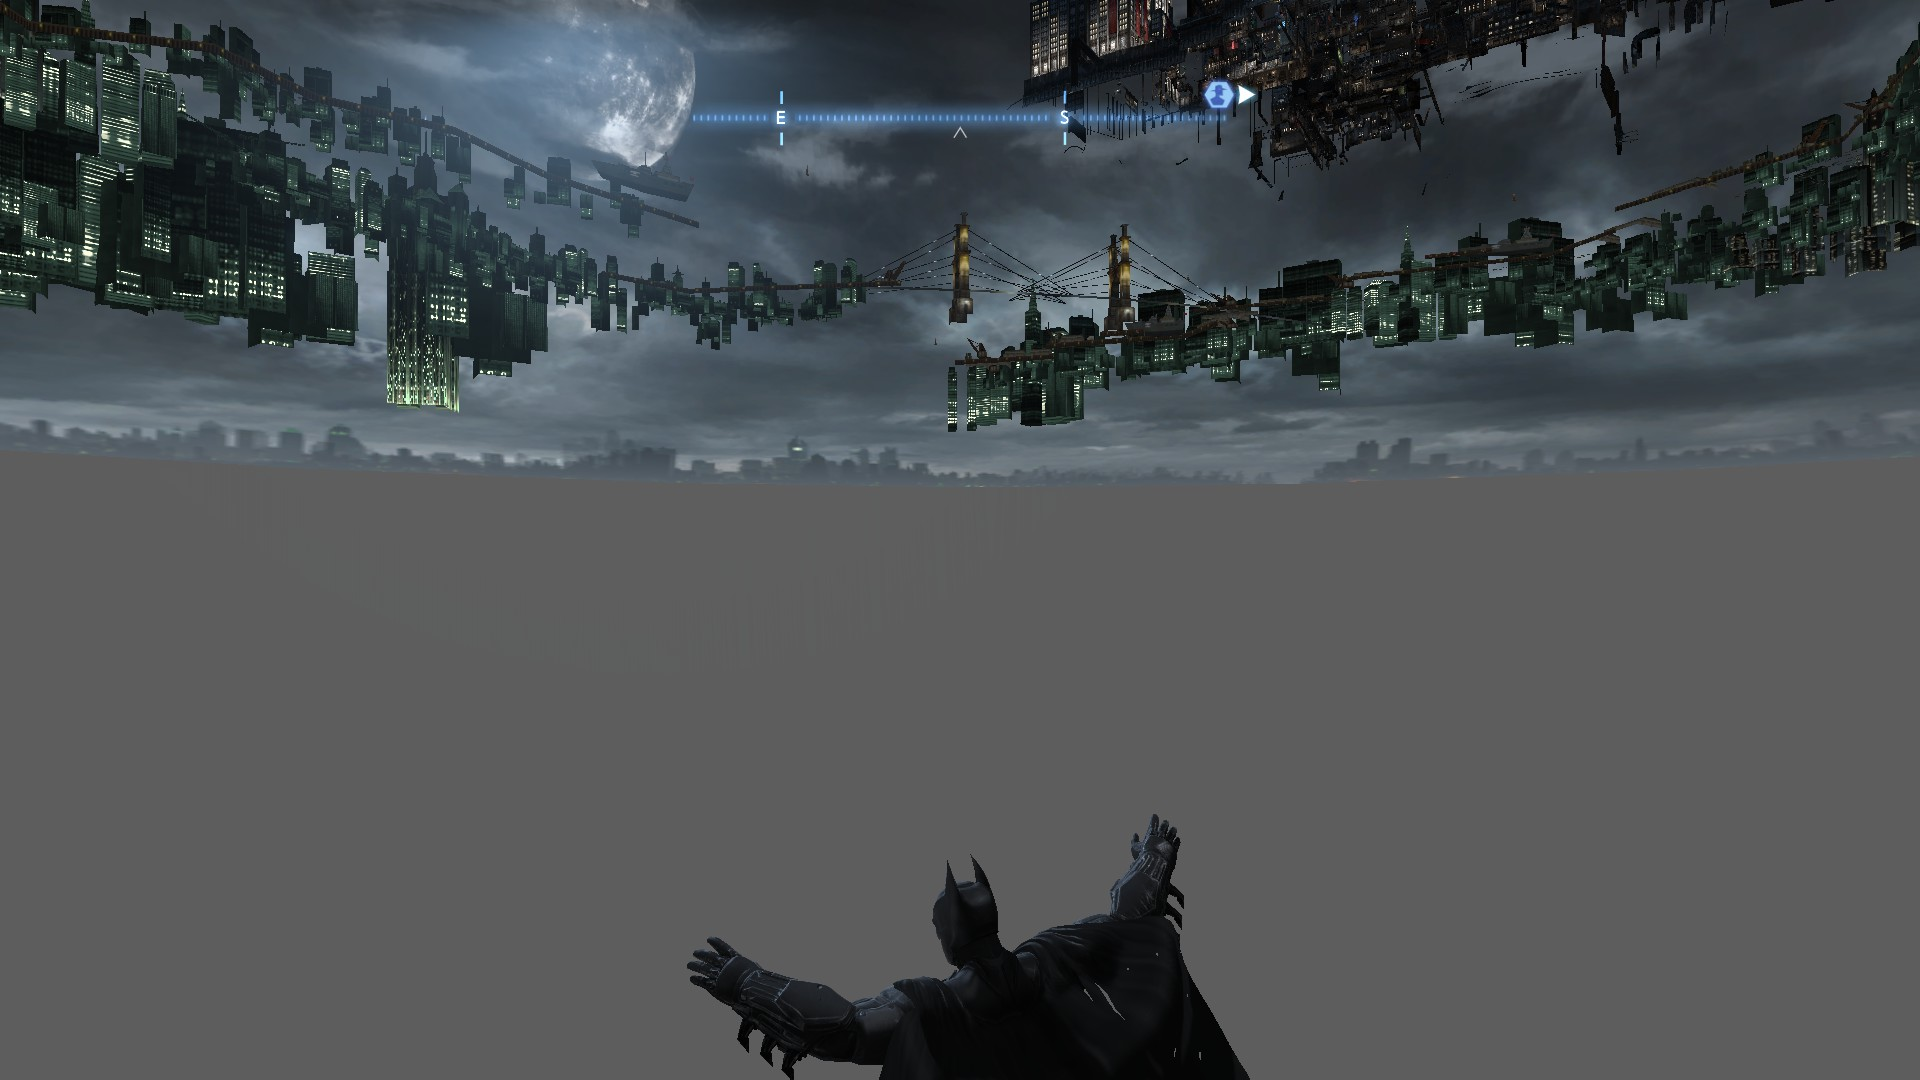
\includegraphics[scale=0.15]{batman.jpg}
\end{center}
\caption{Propadanje kroz mapu.}
\label{fig:batman}
\end{figure}

\begin{figure}[h!]
	\begin{center}
	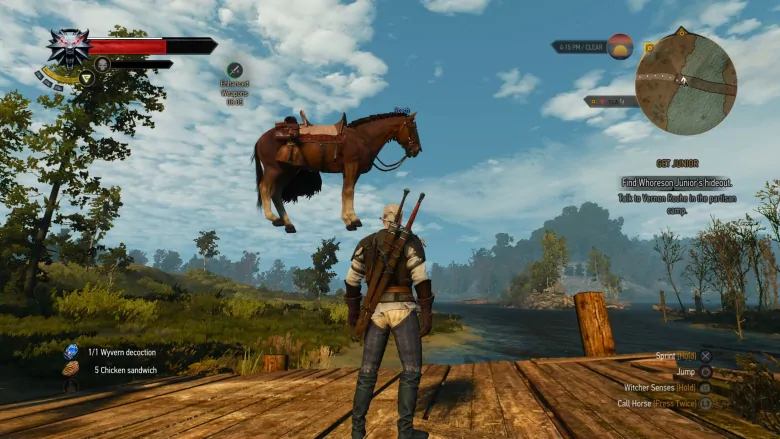
\includegraphics[scale=0.35]{horse.png}
	\end{center}
	\caption{Levitirajući konj.}
	\label{fig:horse}
\end{figure}

Problem detekcije svih parova kolizije je u najgorem slučaju kvadratne složenosti i od toga se ne može pobeći,
ali uglavnom ih ima mnogo manje od gornje granice.
Razlog zahteva da se izvršava u realnom vremenu kod interaktivnih programa je očigledan, ali je takođe
potrebana mogućnost da se što češće i efikasnije utvrde kolizije. Filmovi nisu interaktivan sadržaj i zato
je učestalost osvežavanja slike od 24hz, uz korišćenje zamućivanja pokreta (eng. {\em motion blur}),
dovoljno dobro za većinu ljudi. Standard za igre na konzolama je barem 30hz, a na desktop računarima 
cilj je barem 60hz. Za VR je potrebno barem 90hz inače će lako prouzrokovati dizorijentaciju, mučninu i druge
neželjene efekte \cite{importance}.

Nema najboljeg algoritma detekcije kolizije za svaki mogući slučaj. 
Neki su dobri za uniformno raspoređene objekte u prostoru, ali loši kada su svi na jednom mestu, 
dok su drugi indiferentni što se tiče raspršenosti i više im je bitna brzina kretanja objekata.
Takođe, isti algoritam može imati značajno bolje performanse ako su njegovi parametri dobro 
izabrani za neku hardversku arhitekturu ili scenario. 
Te okolnosti su inspirisale razvoj programa koji omogućava brzo i interaktivno menjanje različitih
algoritama detekcije kolizije, postavljanje njihovih parametara kao i posmatranje performansi.


Ovde pišem tekst. 


\section{Glavne karakteristike}
\label{sec:naslov2}

FPS. 

Konzistentnost fpsa.

Temporalna koherencija.

Paralelizacija, memorija.

Preciznost, preseci zapremina pokretajućih tela.

\section{Neki algoritmi}
\label{sec:algoritmi}


\subsection{Trivijalni}
\label{subsec:octree}


\subsection{Octree}
\label{subsec:octree}


\subsection{Sweep and prune}
\label{subsec:sap}


\subsection{BSP}
\label{subsec:octree}


\section{Implementacija}
\label{sec:implementacija}


\section{Evaluacija}
\label{sec:evaluacija}

\section{Zaključak}
\label{sec:zakljucak}

Zaključak. 

\addcontentsline{toc}{section}{Literatura}
\appendix
\bibliography{bibl} 
\bibliographystyle{plain}

\appendix
\section{Dodatak}
Dodatak.
\end{document}
